\section{Image (d)}

\begin{table}[H]
    \caption{Degrees of each vertex of \cref{fig:graph-d}.}
    \label{tab:graph-d}

    \centering
    \begin{tabular}{ccc}
        \toprule
        \toprule
            Vertex & Degree & Is Odd? \\
        \midrule
            $\hyperlink{fig:graph-d:v1}{v_1}$ & 2 & --- \\
            $\hyperlink{fig:graph-d:v2}{v_2}$ & 2 & --- \\
            $\hyperlink{fig:graph-d:v3}{v_3}$ & 6 & --- \\
            $\hyperlink{fig:graph-d:v4}{v_4}$ & 6 & --- \\
            $\hyperlink{fig:graph-d:v5}{v_5}$ & 3 & Yes \\
            $\hyperlink{fig:graph-d:v6}{v_6}$ & 1 & Yes \\
        \bottomrule
        \bottomrule
    \end{tabular}
\end{table}

\begin{wrapfigure}{r}{0.5\textwidth}
    \centering
    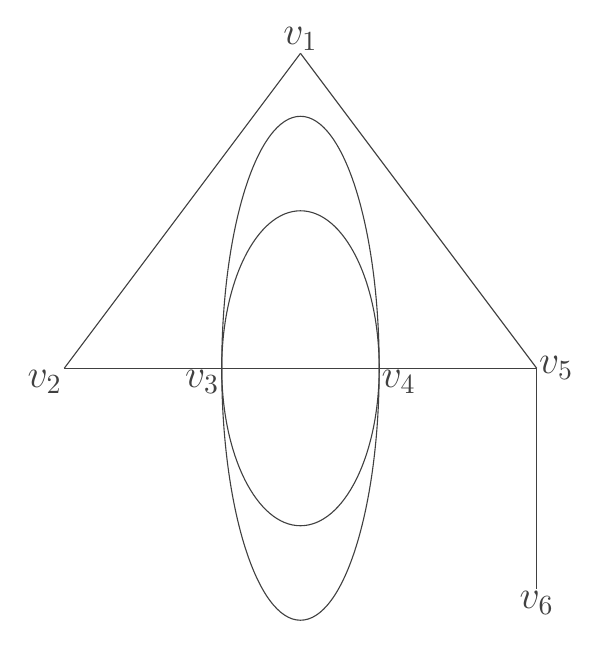
\begin{tikzpicture}[draw=darkgray, text=darkgray, align=center, xscale=1, yscale=2, scale=2]
    \tikzstyle{every node}=[inner sep=0pt];

    \node at ( 0.0, 1) (v1) [label=above:{\Large $v_1$}] {};
    \node at (-1.5, 0) (v2) [label=below left:{\Large $v_2$}] {};
    \node at (-0.5, 0) (v3) [label=below left:{\Large $v_3$}] {};
    \node at ( 0.0, 0) (vc) {};
    \node at ( 0.5, 0) (v4) [label=below right:{\Large $v_4$}] {};
    \node at ( 1.5, 0) (v5) [label=right:{\Large $v_5$}] {};
    \node at ( 1.5, -0.7) (v6) [label=below:{\Large $v_6$}] {};

    \draw (v1.center)
        edge (v2.center);
    \draw (v3.center)
        edge (v2.center)
        edge (v4.center);
    \draw (v5.center)
        edge (v1.center)
        edge (v4.center)
        edge (v6.center);
    \draw (vc.center) ellipse (0.5 and 0.8);
    \draw (vc.center) ellipse (0.5 and 0.5);
\end{tikzpicture}


    \caption{Image \texttt{d.} with labelled nodes.}
    \label{fig:graph-d}
\end{wrapfigure}

Just like with \hyperref[sec:graph-a]{image (a)}, we have exactly two odd vertices, $\hyperlink{fig:graph-d:v5}{v_5}$ and $\hyperlink{fig:graph-d:v6}{v_6}$, in this case. By \cref{thm:euler-trail}, this proves the graph can be drawn as required. As before, both vertices can be used as the starting point for the drawing.
